\documentclass[twoside]{book}

% Packages required by doxygen
\usepackage{fixltx2e}
\usepackage{calc}
\usepackage{doxygen}
\usepackage[export]{adjustbox} % also loads graphicx
\usepackage{graphicx}
\usepackage[utf8]{inputenc}
\usepackage{makeidx}
\usepackage{multicol}
\usepackage{multirow}
\PassOptionsToPackage{warn}{textcomp}
\usepackage{textcomp}
\usepackage[nointegrals]{wasysym}
\usepackage[table]{xcolor}

% Font selection
\usepackage[T1]{fontenc}
\usepackage[scaled=.90]{helvet}
\usepackage{courier}
\usepackage{amssymb}
\usepackage{sectsty}
\renewcommand{\familydefault}{\sfdefault}
\allsectionsfont{%
  \fontseries{bc}\selectfont%
  \color{darkgray}%
}
\renewcommand{\DoxyLabelFont}{%
  \fontseries{bc}\selectfont%
  \color{darkgray}%
}
\newcommand{\+}{\discretionary{\mbox{\scriptsize$\hookleftarrow$}}{}{}}

% Page & text layout
\usepackage{geometry}
\geometry{%
  a4paper,%
  top=2.5cm,%
  bottom=2.5cm,%
  left=2.5cm,%
  right=2.5cm%
}
\tolerance=750
\hfuzz=15pt
\hbadness=750
\setlength{\emergencystretch}{15pt}
\setlength{\parindent}{0cm}
\setlength{\parskip}{3ex plus 2ex minus 2ex}
\makeatletter
\renewcommand{\paragraph}{%
  \@startsection{paragraph}{4}{0ex}{-1.0ex}{1.0ex}{%
    \normalfont\normalsize\bfseries\SS@parafont%
  }%
}
\renewcommand{\subparagraph}{%
  \@startsection{subparagraph}{5}{0ex}{-1.0ex}{1.0ex}{%
    \normalfont\normalsize\bfseries\SS@subparafont%
  }%
}
\makeatother

% Headers & footers
\usepackage{fancyhdr}
\pagestyle{fancyplain}
\fancyhead[LE]{\fancyplain{}{\bfseries\thepage}}
\fancyhead[CE]{\fancyplain{}{}}
\fancyhead[RE]{\fancyplain{}{\bfseries\leftmark}}
\fancyhead[LO]{\fancyplain{}{\bfseries\rightmark}}
\fancyhead[CO]{\fancyplain{}{}}
\fancyhead[RO]{\fancyplain{}{\bfseries\thepage}}
\fancyfoot[LE]{\fancyplain{}{}}
\fancyfoot[CE]{\fancyplain{}{}}
\fancyfoot[RE]{\fancyplain{}{\bfseries\scriptsize Generated by Doxygen }}
\fancyfoot[LO]{\fancyplain{}{\bfseries\scriptsize Generated by Doxygen }}
\fancyfoot[CO]{\fancyplain{}{}}
\fancyfoot[RO]{\fancyplain{}{}}
\renewcommand{\footrulewidth}{0.4pt}
\renewcommand{\chaptermark}[1]{%
  \markboth{#1}{}%
}
\renewcommand{\sectionmark}[1]{%
  \markright{\thesection\ #1}%
}

% Indices & bibliography
\usepackage{natbib}
\usepackage[titles]{tocloft}
\setcounter{tocdepth}{3}
\setcounter{secnumdepth}{5}
\makeindex

% Hyperlinks (required, but should be loaded last)
\usepackage{ifpdf}
\ifpdf
  \usepackage[pdftex,pagebackref=true]{hyperref}
\else
  \usepackage[ps2pdf,pagebackref=true]{hyperref}
\fi
\hypersetup{%
  colorlinks=true,%
  linkcolor=blue,%
  citecolor=blue,%
  unicode%
}

% Custom commands
\newcommand{\clearemptydoublepage}{%
  \newpage{\pagestyle{empty}\cleardoublepage}%
}

\usepackage{caption}
\captionsetup{labelsep=space,justification=centering,font={bf},singlelinecheck=off,skip=4pt,position=top}

%===== C O N T E N T S =====

\begin{document}

% Titlepage & ToC
\hypersetup{pageanchor=false,
             bookmarksnumbered=true,
             pdfencoding=unicode
            }
\pagenumbering{roman}
\begin{titlepage}
\vspace*{7cm}
\begin{center}%
{\Large First Assignment }\\
\vspace*{1cm}
{\large Generated by Doxygen 1.8.11}\\
\end{center}
\end{titlepage}
\clearemptydoublepage
\tableofcontents
\clearemptydoublepage
\pagenumbering{arabic}
\hypersetup{pageanchor=true}

%--- Begin generated contents ---
\chapter{Namespace Index}
\section{Namespace List}
Here is a list of all namespaces with brief descriptions\+:\begin{DoxyCompactList}
\item\contentsline{section}{\hyperlink{namespacebehavior__manager}{behavior\+\_\+manager} \\*Here is implemented the state machine that controls the switch between the behaviours of the robot }{\pageref{namespacebehavior__manager}}{}
\item\contentsline{section}{\hyperlink{namespacemotion}{motion} \\*It moves the robot within the map respecting the behavior }{\pageref{namespacemotion}}{}
\item\contentsline{section}{\hyperlink{namespacepointing__gesture}{pointing\+\_\+gesture} \\*It simulate the pointing gesture command given by the user }{\pageref{namespacepointing__gesture}}{}
\item\contentsline{section}{\hyperlink{namespacevoice__command}{voice\+\_\+command} \\*It simulate the voice commands given by the user }{\pageref{namespacevoice__command}}{}
\end{DoxyCompactList}

\chapter{Hierarchical Index}
\section{Class Hierarchy}
This inheritance list is sorted roughly, but not completely, alphabetically\+:\begin{DoxyCompactList}
\item \contentsline{section}{map2\+Dclass.\+Pet\+Map}{\pageref{classmap2Dclass_1_1PetMap}}{}
\item State\begin{DoxyCompactList}
\item \contentsline{section}{behavior\+\_\+manager.\+Normal\+\_\+behavior}{\pageref{classbehavior__manager_1_1Normal__behavior}}{}
\item \contentsline{section}{behavior\+\_\+manager.\+Play\+\_\+behavior}{\pageref{classbehavior__manager_1_1Play__behavior}}{}
\item \contentsline{section}{behavior\+\_\+manager.\+Sleep\+\_\+behavior}{\pageref{classbehavior__manager_1_1Sleep__behavior}}{}
\end{DoxyCompactList}
\end{DoxyCompactList}

\chapter{Class Index}
\section{Class List}
Here are the classes, structs, unions and interfaces with brief descriptions\+:\begin{DoxyCompactList}
\item\contentsline{section}{\hyperlink{classbehavior__manager_1_1Normal__behavior}{behavior\+\_\+manager.\+Normal\+\_\+behavior} \\*Class \hyperlink{classbehavior__manager_1_1Normal__behavior}{Normal\+\_\+behavior} }{\pageref{classbehavior__manager_1_1Normal__behavior}}{}
\item\contentsline{section}{\hyperlink{classmap2Dclass_1_1PetMap}{map2\+Dclass.\+Pet\+Map} \\*Class Map2D }{\pageref{classmap2Dclass_1_1PetMap}}{}
\item\contentsline{section}{\hyperlink{classbehavior__manager_1_1Play__behavior}{behavior\+\_\+manager.\+Play\+\_\+behavior} \\*Class \hyperlink{classbehavior__manager_1_1Play__behavior}{Play\+\_\+behavior} }{\pageref{classbehavior__manager_1_1Play__behavior}}{}
\item\contentsline{section}{\hyperlink{classbehavior__manager_1_1Sleep__behavior}{behavior\+\_\+manager.\+Sleep\+\_\+behavior} \\*Class \hyperlink{classbehavior__manager_1_1Sleep__behavior}{Sleep\+\_\+behavior} }{\pageref{classbehavior__manager_1_1Sleep__behavior}}{}
\end{DoxyCompactList}

\chapter{File Index}
\section{File List}
Here is a list of all files with brief descriptions\+:\begin{DoxyCompactList}
\item\contentsline{section}{/home/lab\+\_\+exp\+\_\+ws/src/first\+\_\+assignment/src/\hyperlink{behavior__manager_8py}{behavior\+\_\+manager.\+py} }{\pageref{behavior__manager_8py}}{}
\item\contentsline{section}{/home/lab\+\_\+exp\+\_\+ws/src/first\+\_\+assignment/src/\hyperlink{map2D_8py}{map2\+D.\+py} }{\pageref{map2D_8py}}{}
\item\contentsline{section}{/home/lab\+\_\+exp\+\_\+ws/src/first\+\_\+assignment/src/\hyperlink{motion_8py}{motion.\+py} }{\pageref{motion_8py}}{}
\item\contentsline{section}{/home/lab\+\_\+exp\+\_\+ws/src/first\+\_\+assignment/src/\hyperlink{pointing__gesture_8py}{pointing\+\_\+gesture.\+py} }{\pageref{pointing__gesture_8py}}{}
\item\contentsline{section}{/home/lab\+\_\+exp\+\_\+ws/src/first\+\_\+assignment/src/\hyperlink{state__machine__draft_8py}{state\+\_\+machine\+\_\+draft.\+py} }{\pageref{state__machine__draft_8py}}{}
\item\contentsline{section}{/home/lab\+\_\+exp\+\_\+ws/src/first\+\_\+assignment/src/\hyperlink{voice__command_8py}{voice\+\_\+command.\+py} }{\pageref{voice__command_8py}}{}
\end{DoxyCompactList}

\chapter{Namespace Documentation}
\hypertarget{namespacebehavior__manager}{}\section{behavior\+\_\+manager Namespace Reference}
\label{namespacebehavior__manager}\index{behavior\+\_\+manager@{behavior\+\_\+manager}}


Here is implemented the state machine that controls the switch between the behaviours of the robot.  


\subsection*{Classes}
\begin{DoxyCompactItemize}
\item 
class \hyperlink{classbehavior__manager_1_1Normal__behavior}{Normal\+\_\+behavior}
\begin{DoxyCompactList}\small\item\em class \hyperlink{classbehavior__manager_1_1Normal__behavior}{Normal\+\_\+behavior} \end{DoxyCompactList}\item 
class \hyperlink{classbehavior__manager_1_1Play__behavior}{Play\+\_\+behavior}
\begin{DoxyCompactList}\small\item\em class \hyperlink{classbehavior__manager_1_1Play__behavior}{Play\+\_\+behavior} \end{DoxyCompactList}\item 
class \hyperlink{classbehavior__manager_1_1Sleep__behavior}{Sleep\+\_\+behavior}
\begin{DoxyCompactList}\small\item\em class \hyperlink{classbehavior__manager_1_1Sleep__behavior}{Sleep\+\_\+behavior} \end{DoxyCompactList}\end{DoxyCompactItemize}
\subsection*{Functions}
\begin{DoxyCompactItemize}
\item 
def \hyperlink{namespacebehavior__manager_a81416c498199e9a8bc275514afaf9944}{main} ()
\end{DoxyCompactItemize}
\subsection*{Variables}
\begin{DoxyCompactItemize}
\item 
\hyperlink{namespacebehavior__manager_ac30069bca00035c62a13df72bf29a3aa}{pub\+\_\+behavior} = rospy.\+Publisher(\textquotesingle{}/behavior\textquotesingle{}, String, queue\+\_\+size=10)
\end{DoxyCompactItemize}


\subsection{Detailed Description}
Here is implemented the state machine that controls the switch between the behaviours of the robot. 

A finite-\/state machine (F\+SM) is a behavior model that consists of a finite number of states. Based on the current state and a given input the machine performs state transitions and produces outputs The state machine is implemented using the smach library 

\subsection{Function Documentation}
\index{behavior\+\_\+manager@{behavior\+\_\+manager}!main@{main}}
\index{main@{main}!behavior\+\_\+manager@{behavior\+\_\+manager}}
\subsubsection[{\texorpdfstring{main()}{main()}}]{\setlength{\rightskip}{0pt plus 5cm}def behavior\+\_\+manager.\+main (
\begin{DoxyParamCaption}
{}
\end{DoxyParamCaption}
)}\hypertarget{namespacebehavior__manager_a81416c498199e9a8bc275514afaf9944}{}\label{namespacebehavior__manager_a81416c498199e9a8bc275514afaf9944}


\subsection{Variable Documentation}
\index{behavior\+\_\+manager@{behavior\+\_\+manager}!pub\+\_\+behavior@{pub\+\_\+behavior}}
\index{pub\+\_\+behavior@{pub\+\_\+behavior}!behavior\+\_\+manager@{behavior\+\_\+manager}}
\subsubsection[{\texorpdfstring{pub\+\_\+behavior}{pub_behavior}}]{\setlength{\rightskip}{0pt plus 5cm}behavior\+\_\+manager.\+pub\+\_\+behavior = rospy.\+Publisher(\textquotesingle{}/behavior\textquotesingle{}, String, queue\+\_\+size=10)}\hypertarget{namespacebehavior__manager_ac30069bca00035c62a13df72bf29a3aa}{}\label{namespacebehavior__manager_ac30069bca00035c62a13df72bf29a3aa}

\hypertarget{namespacemotion}{}\section{motion Namespace Reference}
\label{namespacemotion}\index{motion@{motion}}


It moves the robot within the map respecting the behavior.  


\subsection*{Functions}
\begin{DoxyCompactItemize}
\item 
def \hyperlink{namespacemotion_a223e65905edcd5f4605198efb23d2ca3}{callback\+\_\+get\+\_\+behaviour} (data)
\begin{DoxyCompactList}\small\item\em callback function callback\+\_\+get\+\_\+behavior \end{DoxyCompactList}\item 
def \hyperlink{namespacemotion_a6fd5e1a0e83ee364babdfa35f8d57076}{update\+\_\+map} (x, y)
\begin{DoxyCompactList}\small\item\em function update\+\_\+map \end{DoxyCompactList}\item 
def \hyperlink{namespacemotion_ab5144d84b423263e4fa8c03c453d975c}{move\+\_\+normal} ()
\begin{DoxyCompactList}\small\item\em function move\+\_\+random \end{DoxyCompactList}\item 
def \hyperlink{namespacemotion_ab22dd13019d977ca14ccf9a84d7f224a}{move\+\_\+reach\+\_\+user} ()
\begin{DoxyCompactList}\small\item\em function move\+\_\+reach\+\_\+user \end{DoxyCompactList}\item 
def \hyperlink{namespacemotion_ad6289fca8572f5af95fd28f4c2dbc68d}{main} ()
\begin{DoxyCompactList}\small\item\em main function \end{DoxyCompactList}\end{DoxyCompactItemize}
\subsection*{Variables}
\begin{DoxyCompactItemize}
\item 
int \hyperlink{namespacemotion_ad15e7b7b1c76162401252ee7533515a4}{xmax} = 30
\item 
int \hyperlink{namespacemotion_a93496959e7cd7b64c958600e13052b02}{ymax} = 30
\item 
int \hyperlink{namespacemotion_a8e0cdf80e6970df1d82ccd96e3f68a1a}{xhome} = 10
\item 
int \hyperlink{namespacemotion_ad24c81915bdf6ae465698c9f63e0c419}{yhome} = 10
\item 
int \hyperlink{namespacemotion_ac1191b288873954280855513ee9ed701}{xuser} = 20
\item 
int \hyperlink{namespacemotion_ae750031c9c1b1e4435481bee11eaf94e}{yuser} = 20
\item 
string \hyperlink{namespacemotion_a24eed052ed35081732fd8920fbbff744}{behaviour} = \char`\"{}play\char`\"{}
\item 
float \hyperlink{namespacemotion_a8b6dad7b29284e6c7e91b64350e3b522}{timescale} = 0.\+5
\end{DoxyCompactItemize}


\subsection{Detailed Description}
It moves the robot within the map respecting the behavior. 

\subsection{Function Documentation}
\index{motion@{motion}!callback\+\_\+get\+\_\+behaviour@{callback\+\_\+get\+\_\+behaviour}}
\index{callback\+\_\+get\+\_\+behaviour@{callback\+\_\+get\+\_\+behaviour}!motion@{motion}}
\subsubsection[{\texorpdfstring{callback\+\_\+get\+\_\+behaviour(data)}{callback_get_behaviour(data)}}]{\setlength{\rightskip}{0pt plus 5cm}def motion.\+callback\+\_\+get\+\_\+behaviour (
\begin{DoxyParamCaption}
\item[{}]{data}
\end{DoxyParamCaption}
)}\hypertarget{namespacemotion_a223e65905edcd5f4605198efb23d2ca3}{}\label{namespacemotion_a223e65905edcd5f4605198efb23d2ca3}


callback function callback\+\_\+get\+\_\+behavior 

subscriber callback to the behaviour topic \index{motion@{motion}!main@{main}}
\index{main@{main}!motion@{motion}}
\subsubsection[{\texorpdfstring{main()}{main()}}]{\setlength{\rightskip}{0pt plus 5cm}def motion.\+main (
\begin{DoxyParamCaption}
{}
\end{DoxyParamCaption}
)}\hypertarget{namespacemotion_ad6289fca8572f5af95fd28f4c2dbc68d}{}\label{namespacemotion_ad6289fca8572f5af95fd28f4c2dbc68d}


main function 

\index{motion@{motion}!move\+\_\+normal@{move\+\_\+normal}}
\index{move\+\_\+normal@{move\+\_\+normal}!motion@{motion}}
\subsubsection[{\texorpdfstring{move\+\_\+normal()}{move_normal()}}]{\setlength{\rightskip}{0pt plus 5cm}def motion.\+move\+\_\+normal (
\begin{DoxyParamCaption}
{}
\end{DoxyParamCaption}
)}\hypertarget{namespacemotion_ab5144d84b423263e4fa8c03c453d975c}{}\label{namespacemotion_ab5144d84b423263e4fa8c03c453d975c}


function move\+\_\+random 

the robot moves randomly when in the N\+O\+R\+M\+AL state \index{motion@{motion}!move\+\_\+reach\+\_\+user@{move\+\_\+reach\+\_\+user}}
\index{move\+\_\+reach\+\_\+user@{move\+\_\+reach\+\_\+user}!motion@{motion}}
\subsubsection[{\texorpdfstring{move\+\_\+reach\+\_\+user()}{move_reach_user()}}]{\setlength{\rightskip}{0pt plus 5cm}def motion.\+move\+\_\+reach\+\_\+user (
\begin{DoxyParamCaption}
{}
\end{DoxyParamCaption}
)}\hypertarget{namespacemotion_ab22dd13019d977ca14ccf9a84d7f224a}{}\label{namespacemotion_ab22dd13019d977ca14ccf9a84d7f224a}


function move\+\_\+reach\+\_\+user 

the robot reached the user when in the P\+L\+AY state \index{motion@{motion}!update\+\_\+map@{update\+\_\+map}}
\index{update\+\_\+map@{update\+\_\+map}!motion@{motion}}
\subsubsection[{\texorpdfstring{update\+\_\+map(x, y)}{update_map(x, y)}}]{\setlength{\rightskip}{0pt plus 5cm}def motion.\+update\+\_\+map (
\begin{DoxyParamCaption}
\item[{}]{x, }
\item[{}]{y}
\end{DoxyParamCaption}
)}\hypertarget{namespacemotion_a6fd5e1a0e83ee364babdfa35f8d57076}{}\label{namespacemotion_a6fd5e1a0e83ee364babdfa35f8d57076}


function update\+\_\+map 

update actual position of the robot with the given one 

\subsection{Variable Documentation}
\index{motion@{motion}!behaviour@{behaviour}}
\index{behaviour@{behaviour}!motion@{motion}}
\subsubsection[{\texorpdfstring{behaviour}{behaviour}}]{\setlength{\rightskip}{0pt plus 5cm}string motion.\+behaviour = \char`\"{}play\char`\"{}}\hypertarget{namespacemotion_a24eed052ed35081732fd8920fbbff744}{}\label{namespacemotion_a24eed052ed35081732fd8920fbbff744}
\index{motion@{motion}!timescale@{timescale}}
\index{timescale@{timescale}!motion@{motion}}
\subsubsection[{\texorpdfstring{timescale}{timescale}}]{\setlength{\rightskip}{0pt plus 5cm}float motion.\+timescale = 0.\+5}\hypertarget{namespacemotion_a8b6dad7b29284e6c7e91b64350e3b522}{}\label{namespacemotion_a8b6dad7b29284e6c7e91b64350e3b522}
\index{motion@{motion}!xhome@{xhome}}
\index{xhome@{xhome}!motion@{motion}}
\subsubsection[{\texorpdfstring{xhome}{xhome}}]{\setlength{\rightskip}{0pt plus 5cm}int motion.\+xhome = 10}\hypertarget{namespacemotion_a8e0cdf80e6970df1d82ccd96e3f68a1a}{}\label{namespacemotion_a8e0cdf80e6970df1d82ccd96e3f68a1a}

\begin{DoxyParams}{Parameters}
{\em xhome} & define X house position for the robot \\
\hline
\end{DoxyParams}
\index{motion@{motion}!xmax@{xmax}}
\index{xmax@{xmax}!motion@{motion}}
\subsubsection[{\texorpdfstring{xmax}{xmax}}]{\setlength{\rightskip}{0pt plus 5cm}int motion.\+xmax = 30}\hypertarget{namespacemotion_ad15e7b7b1c76162401252ee7533515a4}{}\label{namespacemotion_ad15e7b7b1c76162401252ee7533515a4}

\begin{DoxyParams}{Parameters}
{\em xmax} & define max dimension of the map along X \\
\hline
\end{DoxyParams}
\index{motion@{motion}!xuser@{xuser}}
\index{xuser@{xuser}!motion@{motion}}
\subsubsection[{\texorpdfstring{xuser}{xuser}}]{\setlength{\rightskip}{0pt plus 5cm}int motion.\+xuser = 20}\hypertarget{namespacemotion_ac1191b288873954280855513ee9ed701}{}\label{namespacemotion_ac1191b288873954280855513ee9ed701}

\begin{DoxyParams}{Parameters}
{\em xuser} & define X user position for the robot \\
\hline
\end{DoxyParams}
\index{motion@{motion}!yhome@{yhome}}
\index{yhome@{yhome}!motion@{motion}}
\subsubsection[{\texorpdfstring{yhome}{yhome}}]{\setlength{\rightskip}{0pt plus 5cm}int motion.\+yhome = 10}\hypertarget{namespacemotion_ad24c81915bdf6ae465698c9f63e0c419}{}\label{namespacemotion_ad24c81915bdf6ae465698c9f63e0c419}

\begin{DoxyParams}{Parameters}
{\em yhome} & define Y house position for the robot \\
\hline
\end{DoxyParams}
\index{motion@{motion}!ymax@{ymax}}
\index{ymax@{ymax}!motion@{motion}}
\subsubsection[{\texorpdfstring{ymax}{ymax}}]{\setlength{\rightskip}{0pt plus 5cm}int motion.\+ymax = 30}\hypertarget{namespacemotion_a93496959e7cd7b64c958600e13052b02}{}\label{namespacemotion_a93496959e7cd7b64c958600e13052b02}

\begin{DoxyParams}{Parameters}
{\em ymax} & define max dimension of the map along Y \\
\hline
\end{DoxyParams}
\index{motion@{motion}!yuser@{yuser}}
\index{yuser@{yuser}!motion@{motion}}
\subsubsection[{\texorpdfstring{yuser}{yuser}}]{\setlength{\rightskip}{0pt plus 5cm}int motion.\+yuser = 20}\hypertarget{namespacemotion_ae750031c9c1b1e4435481bee11eaf94e}{}\label{namespacemotion_ae750031c9c1b1e4435481bee11eaf94e}

\begin{DoxyParams}{Parameters}
{\em yuser} & define Y user position for the robot \\
\hline
\end{DoxyParams}

\hypertarget{namespacepointing__gesture}{}\section{pointing\+\_\+gesture Namespace Reference}
\label{namespacepointing__gesture}\index{pointing\+\_\+gesture@{pointing\+\_\+gesture}}


It simulate the pointing gesture command given by the user it generates pointing gestures (as Int\+Array) at random times.  


\subsection*{Functions}
\begin{DoxyCompactItemize}
\item 
def \hyperlink{namespacepointing__gesture_a0ccd291e8028504e94f37e49a5411b3d}{callback\+\_\+get\+\_\+behaviour} (data)
\begin{DoxyCompactList}\small\item\em callback function callback\+\_\+get\+\_\+behavior \end{DoxyCompactList}\item 
def \hyperlink{namespacepointing__gesture_a3f243853d60010878f1a2dbbe2338dbd}{compute\+\_\+random\+\_\+position} ()
\begin{DoxyCompactList}\small\item\em function compute\+\_\+random\+\_\+position \end{DoxyCompactList}\item 
def \hyperlink{namespacepointing__gesture_a0246e9d31b3d0b62a01bdb5b697df181}{main} ()
\begin{DoxyCompactList}\small\item\em main function \end{DoxyCompactList}\end{DoxyCompactItemize}
\subsection*{Variables}
\begin{DoxyCompactItemize}
\item 
\hyperlink{namespacepointing__gesture_a16dc32bb0bc4ae96f247e60f4671e69f}{behaviour} = None
\begin{DoxyCompactList}\small\item\em global variables \end{DoxyCompactList}\end{DoxyCompactItemize}


\subsection{Detailed Description}
It simulate the pointing gesture command given by the user it generates pointing gestures (as Int\+Array) at random times. 

\subsection{Function Documentation}
\index{pointing\+\_\+gesture@{pointing\+\_\+gesture}!callback\+\_\+get\+\_\+behaviour@{callback\+\_\+get\+\_\+behaviour}}
\index{callback\+\_\+get\+\_\+behaviour@{callback\+\_\+get\+\_\+behaviour}!pointing\+\_\+gesture@{pointing\+\_\+gesture}}
\subsubsection[{\texorpdfstring{callback\+\_\+get\+\_\+behaviour(data)}{callback_get_behaviour(data)}}]{\setlength{\rightskip}{0pt plus 5cm}def pointing\+\_\+gesture.\+callback\+\_\+get\+\_\+behaviour (
\begin{DoxyParamCaption}
\item[{}]{data}
\end{DoxyParamCaption}
)}\hypertarget{namespacepointing__gesture_a0ccd291e8028504e94f37e49a5411b3d}{}\label{namespacepointing__gesture_a0ccd291e8028504e94f37e49a5411b3d}


callback function callback\+\_\+get\+\_\+behavior 

subscriber callback to the behaviour topic \index{pointing\+\_\+gesture@{pointing\+\_\+gesture}!compute\+\_\+random\+\_\+position@{compute\+\_\+random\+\_\+position}}
\index{compute\+\_\+random\+\_\+position@{compute\+\_\+random\+\_\+position}!pointing\+\_\+gesture@{pointing\+\_\+gesture}}
\subsubsection[{\texorpdfstring{compute\+\_\+random\+\_\+position()}{compute_random_position()}}]{\setlength{\rightskip}{0pt plus 5cm}def pointing\+\_\+gesture.\+compute\+\_\+random\+\_\+position (
\begin{DoxyParamCaption}
{}
\end{DoxyParamCaption}
)}\hypertarget{namespacepointing__gesture_a3f243853d60010878f1a2dbbe2338dbd}{}\label{namespacepointing__gesture_a3f243853d60010878f1a2dbbe2338dbd}


function compute\+\_\+random\+\_\+position 

generate a random position to reach \index{pointing\+\_\+gesture@{pointing\+\_\+gesture}!main@{main}}
\index{main@{main}!pointing\+\_\+gesture@{pointing\+\_\+gesture}}
\subsubsection[{\texorpdfstring{main()}{main()}}]{\setlength{\rightskip}{0pt plus 5cm}def pointing\+\_\+gesture.\+main (
\begin{DoxyParamCaption}
{}
\end{DoxyParamCaption}
)}\hypertarget{namespacepointing__gesture_a0246e9d31b3d0b62a01bdb5b697df181}{}\label{namespacepointing__gesture_a0246e9d31b3d0b62a01bdb5b697df181}


main function 



\subsection{Variable Documentation}
\index{pointing\+\_\+gesture@{pointing\+\_\+gesture}!behaviour@{behaviour}}
\index{behaviour@{behaviour}!pointing\+\_\+gesture@{pointing\+\_\+gesture}}
\subsubsection[{\texorpdfstring{behaviour}{behaviour}}]{\setlength{\rightskip}{0pt plus 5cm}pointing\+\_\+gesture.\+behaviour = None}\hypertarget{namespacepointing__gesture_a16dc32bb0bc4ae96f247e60f4671e69f}{}\label{namespacepointing__gesture_a16dc32bb0bc4ae96f247e60f4671e69f}


global variables 


\hypertarget{namespacevoice__command}{}\section{voice\+\_\+command Namespace Reference}
\label{namespacevoice__command}\index{voice\+\_\+command@{voice\+\_\+command}}


It simulate the voice commands given by the user.  




\subsection{Detailed Description}
It simulate the voice commands given by the user. 
\chapter{Class Documentation}
\hypertarget{classbehavior__manager_1_1Normal__behavior}{}\section{behavior\+\_\+manager.\+Normal\+\_\+behavior Class Reference}
\label{classbehavior__manager_1_1Normal__behavior}\index{behavior\+\_\+manager.\+Normal\+\_\+behavior@{behavior\+\_\+manager.\+Normal\+\_\+behavior}}


class \hyperlink{classbehavior__manager_1_1Normal__behavior}{Normal\+\_\+behavior}  




Inheritance diagram for behavior\+\_\+manager.\+Normal\+\_\+behavior\+:\nopagebreak
\begin{figure}[H]
\begin{center}
\leavevmode
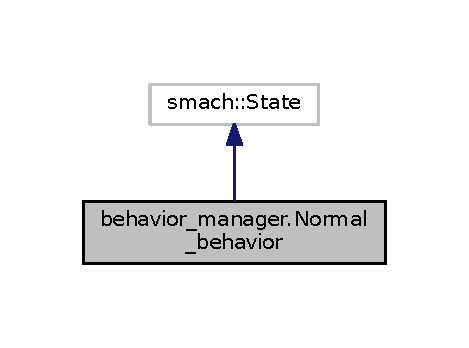
\includegraphics[width=225pt]{classbehavior__manager_1_1Normal__behavior__inherit__graph}
\end{center}
\end{figure}


Collaboration diagram for behavior\+\_\+manager.\+Normal\+\_\+behavior\+:\nopagebreak
\begin{figure}[H]
\begin{center}
\leavevmode
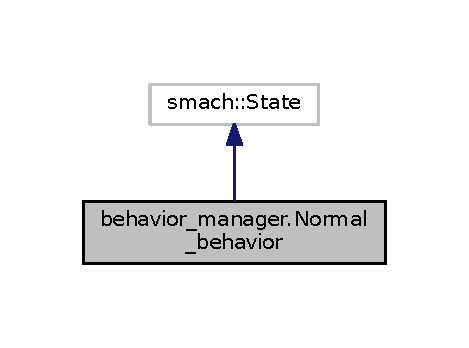
\includegraphics[width=225pt]{classbehavior__manager_1_1Normal__behavior__coll__graph}
\end{center}
\end{figure}
\subsection*{Public Member Functions}
\begin{DoxyCompactItemize}
\item 
def \hyperlink{classbehavior__manager_1_1Normal__behavior_a7ab22900e936fc3921a269389b51e6ab}{\+\_\+\+\_\+init\+\_\+\+\_\+} (self)
\begin{DoxyCompactList}\small\item\em method init \end{DoxyCompactList}\item 
def \hyperlink{classbehavior__manager_1_1Normal__behavior_a15faab6a43a39510355baad4faaa808a}{execute} (self, userdata)
\begin{DoxyCompactList}\small\item\em method execute \end{DoxyCompactList}\item 
def \hyperlink{classbehavior__manager_1_1Normal__behavior_aaaac0d8e5b98600a4e8461f706cb7ef0}{get\+\_\+command} (self, command)
\begin{DoxyCompactList}\small\item\em method get\+\_\+command \end{DoxyCompactList}\end{DoxyCompactItemize}
\subsection*{Public Attributes}
\begin{DoxyCompactItemize}
\item 
\hyperlink{classbehavior__manager_1_1Normal__behavior_a023e0b91a5c02b8bce8cc771bba4ecfc}{play\+\_\+command\+\_\+received}
\begin{DoxyCompactList}\small\item\em check if the user command is received, subscribe to the topic \hyperlink{namespacevoice__command}{voice\+\_\+command} on which \hyperlink{voice__command_8py}{voice\+\_\+command.\+py} publishes \char`\"{}play\char`\"{} \end{DoxyCompactList}\item 
\hyperlink{classbehavior__manager_1_1Normal__behavior_a8c0881c34370caec4f5298f0ebe35489}{rate}
\end{DoxyCompactItemize}


\subsection{Detailed Description}
class \hyperlink{classbehavior__manager_1_1Normal__behavior}{Normal\+\_\+behavior} 

This class implement the N\+O\+R\+M\+AL behaviour of the robot pet The robot moves randomly within the map
\begin{DoxyItemize}
\item If it receives a \char`\"{}play\char`\"{} command the F\+SM should go into P\+L\+AY state
\item If the sleep timer is triggered the F\+SM should go into S\+L\+E\+EP state 
\end{DoxyItemize}

\subsection{Constructor \& Destructor Documentation}
\index{behavior\+\_\+manager\+::\+Normal\+\_\+behavior@{behavior\+\_\+manager\+::\+Normal\+\_\+behavior}!\+\_\+\+\_\+init\+\_\+\+\_\+@{\+\_\+\+\_\+init\+\_\+\+\_\+}}
\index{\+\_\+\+\_\+init\+\_\+\+\_\+@{\+\_\+\+\_\+init\+\_\+\+\_\+}!behavior\+\_\+manager\+::\+Normal\+\_\+behavior@{behavior\+\_\+manager\+::\+Normal\+\_\+behavior}}
\subsubsection[{\texorpdfstring{\+\_\+\+\_\+init\+\_\+\+\_\+(self)}{__init__(self)}}]{\setlength{\rightskip}{0pt plus 5cm}def behavior\+\_\+manager.\+Normal\+\_\+behavior.\+\_\+\+\_\+init\+\_\+\+\_\+ (
\begin{DoxyParamCaption}
\item[{}]{self}
\end{DoxyParamCaption}
)}\hypertarget{classbehavior__manager_1_1Normal__behavior_a7ab22900e936fc3921a269389b51e6ab}{}\label{classbehavior__manager_1_1Normal__behavior_a7ab22900e936fc3921a269389b51e6ab}


method init 

it initializes the state class 

\subsection{Member Function Documentation}
\index{behavior\+\_\+manager\+::\+Normal\+\_\+behavior@{behavior\+\_\+manager\+::\+Normal\+\_\+behavior}!execute@{execute}}
\index{execute@{execute}!behavior\+\_\+manager\+::\+Normal\+\_\+behavior@{behavior\+\_\+manager\+::\+Normal\+\_\+behavior}}
\subsubsection[{\texorpdfstring{execute(self, userdata)}{execute(self, userdata)}}]{\setlength{\rightskip}{0pt plus 5cm}def behavior\+\_\+manager.\+Normal\+\_\+behavior.\+execute (
\begin{DoxyParamCaption}
\item[{}]{self, }
\item[{}]{userdata}
\end{DoxyParamCaption}
)}\hypertarget{classbehavior__manager_1_1Normal__behavior_a15faab6a43a39510355baad4faaa808a}{}\label{classbehavior__manager_1_1Normal__behavior_a15faab6a43a39510355baad4faaa808a}


method execute 


\begin{DoxyItemize}
\item publish \char`\"{}normal\char`\"{} (String) on the topic behavior
\item check if a voice command is received from the user
\item if the command is received\+:
\begin{DoxyItemize}
\item goes into P\+L\+AY state
\end{DoxyItemize}
\item else
\begin{DoxyItemize}
\item trigger sleeping timer at random time
\item goes into S\+L\+E\+EP state 
\end{DoxyItemize}
\end{DoxyItemize}\index{behavior\+\_\+manager\+::\+Normal\+\_\+behavior@{behavior\+\_\+manager\+::\+Normal\+\_\+behavior}!get\+\_\+command@{get\+\_\+command}}
\index{get\+\_\+command@{get\+\_\+command}!behavior\+\_\+manager\+::\+Normal\+\_\+behavior@{behavior\+\_\+manager\+::\+Normal\+\_\+behavior}}
\subsubsection[{\texorpdfstring{get\+\_\+command(self, command)}{get_command(self, command)}}]{\setlength{\rightskip}{0pt plus 5cm}def behavior\+\_\+manager.\+Normal\+\_\+behavior.\+get\+\_\+command (
\begin{DoxyParamCaption}
\item[{}]{self, }
\item[{}]{command}
\end{DoxyParamCaption}
)}\hypertarget{classbehavior__manager_1_1Normal__behavior_aaaac0d8e5b98600a4e8461f706cb7ef0}{}\label{classbehavior__manager_1_1Normal__behavior_aaaac0d8e5b98600a4e8461f706cb7ef0}


method get\+\_\+command 

method to get the voice command 

\subsection{Member Data Documentation}
\index{behavior\+\_\+manager\+::\+Normal\+\_\+behavior@{behavior\+\_\+manager\+::\+Normal\+\_\+behavior}!play\+\_\+command\+\_\+received@{play\+\_\+command\+\_\+received}}
\index{play\+\_\+command\+\_\+received@{play\+\_\+command\+\_\+received}!behavior\+\_\+manager\+::\+Normal\+\_\+behavior@{behavior\+\_\+manager\+::\+Normal\+\_\+behavior}}
\subsubsection[{\texorpdfstring{play\+\_\+command\+\_\+received}{play_command_received}}]{\setlength{\rightskip}{0pt plus 5cm}behavior\+\_\+manager.\+Normal\+\_\+behavior.\+play\+\_\+command\+\_\+received}\hypertarget{classbehavior__manager_1_1Normal__behavior_a023e0b91a5c02b8bce8cc771bba4ecfc}{}\label{classbehavior__manager_1_1Normal__behavior_a023e0b91a5c02b8bce8cc771bba4ecfc}


check if the user command is received, subscribe to the topic \hyperlink{namespacevoice__command}{voice\+\_\+command} on which \hyperlink{voice__command_8py}{voice\+\_\+command.\+py} publishes \char`\"{}play\char`\"{} 

wait random time \index{behavior\+\_\+manager\+::\+Normal\+\_\+behavior@{behavior\+\_\+manager\+::\+Normal\+\_\+behavior}!rate@{rate}}
\index{rate@{rate}!behavior\+\_\+manager\+::\+Normal\+\_\+behavior@{behavior\+\_\+manager\+::\+Normal\+\_\+behavior}}
\subsubsection[{\texorpdfstring{rate}{rate}}]{\setlength{\rightskip}{0pt plus 5cm}behavior\+\_\+manager.\+Normal\+\_\+behavior.\+rate}\hypertarget{classbehavior__manager_1_1Normal__behavior_a8c0881c34370caec4f5298f0ebe35489}{}\label{classbehavior__manager_1_1Normal__behavior_a8c0881c34370caec4f5298f0ebe35489}


The documentation for this class was generated from the following file\+:\begin{DoxyCompactItemize}
\item 
/home/lab\+\_\+exp\+\_\+ws/src/first\+\_\+assignment/src/\hyperlink{behavior__manager_8py}{behavior\+\_\+manager.\+py}\end{DoxyCompactItemize}

\hypertarget{classbehavior__manager_1_1Play__behavior}{}\section{behavior\+\_\+manager.\+Play\+\_\+behavior Class Reference}
\label{classbehavior__manager_1_1Play__behavior}\index{behavior\+\_\+manager.\+Play\+\_\+behavior@{behavior\+\_\+manager.\+Play\+\_\+behavior}}


class \hyperlink{classbehavior__manager_1_1Play__behavior}{Play\+\_\+behavior}  




Inheritance diagram for behavior\+\_\+manager.\+Play\+\_\+behavior\+:\nopagebreak
\begin{figure}[H]
\begin{center}
\leavevmode
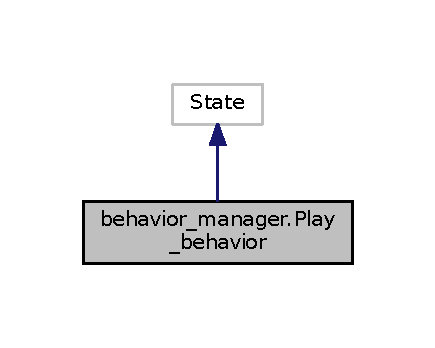
\includegraphics[width=209pt]{classbehavior__manager_1_1Play__behavior__inherit__graph}
\end{center}
\end{figure}


Collaboration diagram for behavior\+\_\+manager.\+Play\+\_\+behavior\+:\nopagebreak
\begin{figure}[H]
\begin{center}
\leavevmode
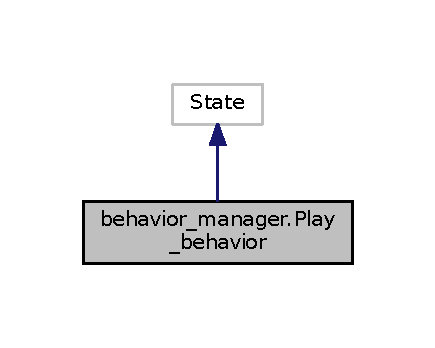
\includegraphics[width=209pt]{classbehavior__manager_1_1Play__behavior__coll__graph}
\end{center}
\end{figure}
\subsection*{Public Member Functions}
\begin{DoxyCompactItemize}
\item 
def \hyperlink{classbehavior__manager_1_1Play__behavior_aaa6ce2b1855d0a235e324df41d8519a1}{\+\_\+\+\_\+init\+\_\+\+\_\+} (self)
\begin{DoxyCompactList}\small\item\em method init \end{DoxyCompactList}\item 
def \hyperlink{classbehavior__manager_1_1Play__behavior_a6c5231ed8f406c82e06c741e89b0f666}{execute} (self, userdata)
\begin{DoxyCompactList}\small\item\em method execute \end{DoxyCompactList}\end{DoxyCompactItemize}


\subsection{Detailed Description}
class \hyperlink{classbehavior__manager_1_1Play__behavior}{Play\+\_\+behavior} 

This class implement the P\+L\+AY behaviour of the robot pet 

\subsection{Constructor \& Destructor Documentation}
\index{behavior\+\_\+manager\+::\+Play\+\_\+behavior@{behavior\+\_\+manager\+::\+Play\+\_\+behavior}!\+\_\+\+\_\+init\+\_\+\+\_\+@{\+\_\+\+\_\+init\+\_\+\+\_\+}}
\index{\+\_\+\+\_\+init\+\_\+\+\_\+@{\+\_\+\+\_\+init\+\_\+\+\_\+}!behavior\+\_\+manager\+::\+Play\+\_\+behavior@{behavior\+\_\+manager\+::\+Play\+\_\+behavior}}
\subsubsection[{\texorpdfstring{\+\_\+\+\_\+init\+\_\+\+\_\+(self)}{__init__(self)}}]{\setlength{\rightskip}{0pt plus 5cm}def behavior\+\_\+manager.\+Play\+\_\+behavior.\+\_\+\+\_\+init\+\_\+\+\_\+ (
\begin{DoxyParamCaption}
\item[{}]{self}
\end{DoxyParamCaption}
)}\hypertarget{classbehavior__manager_1_1Play__behavior_aaa6ce2b1855d0a235e324df41d8519a1}{}\label{classbehavior__manager_1_1Play__behavior_aaa6ce2b1855d0a235e324df41d8519a1}


method init 

it initializes the state class 

\subsection{Member Function Documentation}
\index{behavior\+\_\+manager\+::\+Play\+\_\+behavior@{behavior\+\_\+manager\+::\+Play\+\_\+behavior}!execute@{execute}}
\index{execute@{execute}!behavior\+\_\+manager\+::\+Play\+\_\+behavior@{behavior\+\_\+manager\+::\+Play\+\_\+behavior}}
\subsubsection[{\texorpdfstring{execute(self, userdata)}{execute(self, userdata)}}]{\setlength{\rightskip}{0pt plus 5cm}def behavior\+\_\+manager.\+Play\+\_\+behavior.\+execute (
\begin{DoxyParamCaption}
\item[{}]{self, }
\item[{}]{userdata}
\end{DoxyParamCaption}
)}\hypertarget{classbehavior__manager_1_1Play__behavior_a6c5231ed8f406c82e06c741e89b0f666}{}\label{classbehavior__manager_1_1Play__behavior_a6c5231ed8f406c82e06c741e89b0f666}


method execute 

it executes the required actions 

The documentation for this class was generated from the following file\+:\begin{DoxyCompactItemize}
\item 
/home/lab\+\_\+exp\+\_\+ws/src/first\+\_\+assignment/src/\hyperlink{behavior__manager_8py}{behavior\+\_\+manager.\+py}\end{DoxyCompactItemize}

\hypertarget{classbehavior__manager_1_1Sleep__behavior}{}\section{behavior\+\_\+manager.\+Sleep\+\_\+behavior Class Reference}
\label{classbehavior__manager_1_1Sleep__behavior}\index{behavior\+\_\+manager.\+Sleep\+\_\+behavior@{behavior\+\_\+manager.\+Sleep\+\_\+behavior}}


class \hyperlink{classbehavior__manager_1_1Sleep__behavior}{Sleep\+\_\+behavior}  




Inheritance diagram for behavior\+\_\+manager.\+Sleep\+\_\+behavior\+:\nopagebreak
\begin{figure}[H]
\begin{center}
\leavevmode
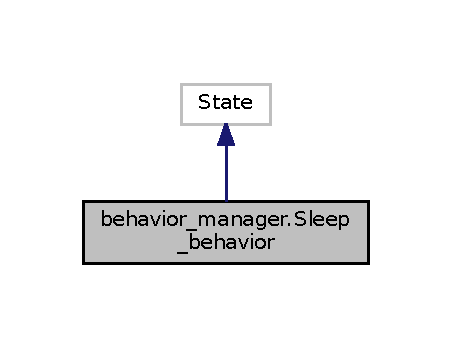
\includegraphics[width=217pt]{classbehavior__manager_1_1Sleep__behavior__inherit__graph}
\end{center}
\end{figure}


Collaboration diagram for behavior\+\_\+manager.\+Sleep\+\_\+behavior\+:\nopagebreak
\begin{figure}[H]
\begin{center}
\leavevmode
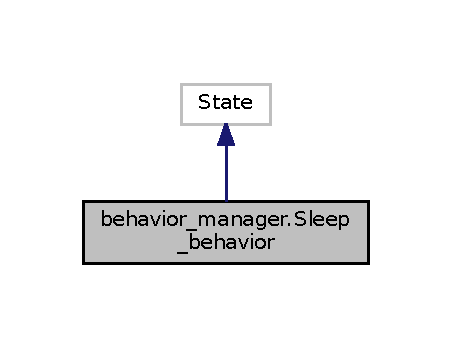
\includegraphics[width=217pt]{classbehavior__manager_1_1Sleep__behavior__coll__graph}
\end{center}
\end{figure}
\subsection*{Public Member Functions}
\begin{DoxyCompactItemize}
\item 
def \hyperlink{classbehavior__manager_1_1Sleep__behavior_a778df3c5a36999ef4792e6ac444bd7f3}{\+\_\+\+\_\+init\+\_\+\+\_\+} (self)
\begin{DoxyCompactList}\small\item\em method init \end{DoxyCompactList}\item 
def \hyperlink{classbehavior__manager_1_1Sleep__behavior_a02d87859cb76d2dbdf78d9d6e2452782}{execute} (self, userdata)
\begin{DoxyCompactList}\small\item\em method execute \end{DoxyCompactList}\end{DoxyCompactItemize}


\subsection{Detailed Description}
class \hyperlink{classbehavior__manager_1_1Sleep__behavior}{Sleep\+\_\+behavior} 

This class implement the S\+L\+E\+EP behaviour of the robot pet The robot sleeps (S\+L\+E\+EP state)for a random period of time, then it moves to N\+O\+R\+M\+AL state 

\subsection{Constructor \& Destructor Documentation}
\index{behavior\+\_\+manager\+::\+Sleep\+\_\+behavior@{behavior\+\_\+manager\+::\+Sleep\+\_\+behavior}!\+\_\+\+\_\+init\+\_\+\+\_\+@{\+\_\+\+\_\+init\+\_\+\+\_\+}}
\index{\+\_\+\+\_\+init\+\_\+\+\_\+@{\+\_\+\+\_\+init\+\_\+\+\_\+}!behavior\+\_\+manager\+::\+Sleep\+\_\+behavior@{behavior\+\_\+manager\+::\+Sleep\+\_\+behavior}}
\subsubsection[{\texorpdfstring{\+\_\+\+\_\+init\+\_\+\+\_\+(self)}{__init__(self)}}]{\setlength{\rightskip}{0pt plus 5cm}def behavior\+\_\+manager.\+Sleep\+\_\+behavior.\+\_\+\+\_\+init\+\_\+\+\_\+ (
\begin{DoxyParamCaption}
\item[{}]{self}
\end{DoxyParamCaption}
)}\hypertarget{classbehavior__manager_1_1Sleep__behavior_a778df3c5a36999ef4792e6ac444bd7f3}{}\label{classbehavior__manager_1_1Sleep__behavior_a778df3c5a36999ef4792e6ac444bd7f3}


method init 

it initializes the state class 

\subsection{Member Function Documentation}
\index{behavior\+\_\+manager\+::\+Sleep\+\_\+behavior@{behavior\+\_\+manager\+::\+Sleep\+\_\+behavior}!execute@{execute}}
\index{execute@{execute}!behavior\+\_\+manager\+::\+Sleep\+\_\+behavior@{behavior\+\_\+manager\+::\+Sleep\+\_\+behavior}}
\subsubsection[{\texorpdfstring{execute(self, userdata)}{execute(self, userdata)}}]{\setlength{\rightskip}{0pt plus 5cm}def behavior\+\_\+manager.\+Sleep\+\_\+behavior.\+execute (
\begin{DoxyParamCaption}
\item[{}]{self, }
\item[{}]{userdata}
\end{DoxyParamCaption}
)}\hypertarget{classbehavior__manager_1_1Sleep__behavior_a02d87859cb76d2dbdf78d9d6e2452782}{}\label{classbehavior__manager_1_1Sleep__behavior_a02d87859cb76d2dbdf78d9d6e2452782}


method execute 

it executes the required actions 

The documentation for this class was generated from the following file\+:\begin{DoxyCompactItemize}
\item 
/home/lab\+\_\+exp\+\_\+ws/src/first\+\_\+assignment/src/\hyperlink{behavior__manager_8py}{behavior\+\_\+manager.\+py}\end{DoxyCompactItemize}

\chapter{File Documentation}
\hypertarget{behavior__manager_8py}{}\section{/home/lab\+\_\+exp\+\_\+ws/src/first\+\_\+assignment/src/behavior\+\_\+manager.py File Reference}
\label{behavior__manager_8py}\index{/home/lab\+\_\+exp\+\_\+ws/src/first\+\_\+assignment/src/behavior\+\_\+manager.\+py@{/home/lab\+\_\+exp\+\_\+ws/src/first\+\_\+assignment/src/behavior\+\_\+manager.\+py}}
\subsection*{Classes}
\begin{DoxyCompactItemize}
\item 
class \hyperlink{classbehavior__manager_1_1Normal__behavior}{behavior\+\_\+manager.\+Normal\+\_\+behavior}
\begin{DoxyCompactList}\small\item\em class \hyperlink{classbehavior__manager_1_1Normal__behavior}{Normal\+\_\+behavior} \end{DoxyCompactList}\item 
class \hyperlink{classbehavior__manager_1_1Sleep__behavior}{behavior\+\_\+manager.\+Sleep\+\_\+behavior}
\begin{DoxyCompactList}\small\item\em class \hyperlink{classbehavior__manager_1_1Sleep__behavior}{Sleep\+\_\+behavior} \end{DoxyCompactList}\item 
class \hyperlink{classbehavior__manager_1_1Play__behavior}{behavior\+\_\+manager.\+Play\+\_\+behavior}
\begin{DoxyCompactList}\small\item\em class \hyperlink{classbehavior__manager_1_1Play__behavior}{Play\+\_\+behavior} \end{DoxyCompactList}\end{DoxyCompactItemize}
\subsection*{Namespaces}
\begin{DoxyCompactItemize}
\item 
 \hyperlink{namespacebehavior__manager}{behavior\+\_\+manager}
\begin{DoxyCompactList}\small\item\em Here is implemented the state machine that controls the switch between the behaviours of the robot. \end{DoxyCompactList}\end{DoxyCompactItemize}
\subsection*{Functions}
\begin{DoxyCompactItemize}
\item 
def \hyperlink{namespacebehavior__manager_a81416c498199e9a8bc275514afaf9944}{behavior\+\_\+manager.\+main} ()
\end{DoxyCompactItemize}
\subsection*{Variables}
\begin{DoxyCompactItemize}
\item 
float \hyperlink{namespacebehavior__manager_a53d496c1cdb4a1a21f698d78a6baeb6e}{behavior\+\_\+manager.\+random\+\_\+time} = 0.\+5
\begin{DoxyCompactList}\small\item\em global variables \end{DoxyCompactList}\item 
int \hyperlink{namespacebehavior__manager_a49c9b541017b9483f311fd59e6f7fec6}{behavior\+\_\+manager.\+xhome} = 10
\item 
int \hyperlink{namespacebehavior__manager_a8a02239f22d228c9aea6e13b43a5cdee}{behavior\+\_\+manager.\+yhome} = 10
\item 
\hyperlink{namespacebehavior__manager_ac30069bca00035c62a13df72bf29a3aa}{behavior\+\_\+manager.\+pub\+\_\+behavior} = rospy.\+Publisher(\textquotesingle{}/behavior\textquotesingle{}, String, queue\+\_\+size=10)
\begin{DoxyCompactList}\small\item\em publisher pub\+\_\+behavior \end{DoxyCompactList}\end{DoxyCompactItemize}

\hypertarget{motion_8py}{}\section{/home/lab\+\_\+exp\+\_\+ws/src/first\+\_\+assignment/src/motion.py File Reference}
\label{motion_8py}\index{/home/lab\+\_\+exp\+\_\+ws/src/first\+\_\+assignment/src/motion.\+py@{/home/lab\+\_\+exp\+\_\+ws/src/first\+\_\+assignment/src/motion.\+py}}
\subsection*{Namespaces}
\begin{DoxyCompactItemize}
\item 
 \hyperlink{namespacemotion}{motion}
\begin{DoxyCompactList}\small\item\em It moves the robot within the map respecting the behavior. \end{DoxyCompactList}\end{DoxyCompactItemize}
\subsection*{Functions}
\begin{DoxyCompactItemize}
\item 
def \hyperlink{namespacemotion_a223e65905edcd5f4605198efb23d2ca3}{motion.\+callback\+\_\+get\+\_\+behaviour} (data)
\begin{DoxyCompactList}\small\item\em callback function callback\+\_\+get\+\_\+behavior \end{DoxyCompactList}\item 
def \hyperlink{namespacemotion_a9a93c5fd6c8938302c99cdc865f34cb8}{motion.\+update\+\_\+position} (x, y)
\begin{DoxyCompactList}\small\item\em function update\+\_\+position \end{DoxyCompactList}\item 
def \hyperlink{namespacemotion_ab5144d84b423263e4fa8c03c453d975c}{motion.\+move\+\_\+normal} ()
\begin{DoxyCompactList}\small\item\em function move\+\_\+random \end{DoxyCompactList}\item 
def \hyperlink{namespacemotion_ab22dd13019d977ca14ccf9a84d7f224a}{motion.\+move\+\_\+reach\+\_\+user} ()
\begin{DoxyCompactList}\small\item\em function move\+\_\+reach\+\_\+user \end{DoxyCompactList}\item 
def \hyperlink{namespacemotion_a7e28371ac015cdd23c39095626abce98}{motion.\+move\+\_\+sleep\+\_\+position} ()
\begin{DoxyCompactList}\small\item\em function move\+\_\+sleep\+\_\+position \end{DoxyCompactList}\item 
def \hyperlink{namespacemotion_aea14bdb6100f2e8e6035a4487c861bc7}{motion.\+callback\+\_\+get\+\_\+position} (position)
\begin{DoxyCompactList}\small\item\em function callback\+\_\+get\+\_\+position \end{DoxyCompactList}\item 
def \hyperlink{namespacemotion_a58accc2356096af3ae30fe9442a1a482}{motion.\+reach\+\_\+goal} ()
\begin{DoxyCompactList}\small\item\em function reach\+\_\+goal \end{DoxyCompactList}\item 
def \hyperlink{namespacemotion_ad6289fca8572f5af95fd28f4c2dbc68d}{motion.\+main} ()
\begin{DoxyCompactList}\small\item\em main function \end{DoxyCompactList}\end{DoxyCompactItemize}
\subsection*{Variables}
\begin{DoxyCompactItemize}
\item 
\hyperlink{namespacemotion_a15d63b2a70ac940f179085ce72871c86}{motion.\+behaviour} = None
\begin{DoxyCompactList}\small\item\em all these param are now saved in the class Map2D in \hyperlink{map2Dclass_8py}{map2\+Dclass.\+py} xmax define max dimension of the map along X xmax = 30 ymax define max dimension of the map along Y ymax = 30 xhome define X house position for the robot xhome = 10 yhome define Y house position for the robot yhome = 10 xuser define X user position for the robot xuser = 20 yuser define Y user position for the robot yuser = 20 \end{DoxyCompactList}\item 
bool \hyperlink{namespacemotion_a30e58643e988d1faddb84cdfd54965f8}{motion.\+at\+\_\+home} = False
\item 
\hyperlink{namespacemotion_a6427953689c120f9b8a1cb3646733b85}{motion.\+goal} = None
\item 
float \hyperlink{namespacemotion_a577a5f71c1bdf849f48eed17c4134bee}{motion.\+random\+\_\+time} = 0.\+5
\item 
\hyperlink{namespacemotion_a858c2a633daaa0a83b599397041f524b}{motion.\+map\+\_\+2D} = Map2D()
\begin{DoxyCompactList}\small\item\em object for access the values of the map2D \end{DoxyCompactList}\item 
\hyperlink{namespacemotion_a9213de80f34f408518c9265ee283b588}{motion.\+pub\+\_\+actual} = rospy.\+Publisher(\char`\"{}/actual\+\_\+position\+\_\+robot\char`\"{},Int\+Array,queue\+\_\+size=10)
\begin{DoxyCompactList}\small\item\em publisher of actual position of the robot \end{DoxyCompactList}\end{DoxyCompactItemize}

\hypertarget{pointing__gesture_8py}{}\section{/home/lab\+\_\+exp\+\_\+ws/src/first\+\_\+assignment/src/pointing\+\_\+gesture.py File Reference}
\label{pointing__gesture_8py}\index{/home/lab\+\_\+exp\+\_\+ws/src/first\+\_\+assignment/src/pointing\+\_\+gesture.\+py@{/home/lab\+\_\+exp\+\_\+ws/src/first\+\_\+assignment/src/pointing\+\_\+gesture.\+py}}
\subsection*{Namespaces}
\begin{DoxyCompactItemize}
\item 
 \hyperlink{namespacepointing__gesture}{pointing\+\_\+gesture}
\begin{DoxyCompactList}\small\item\em It simulate the pointing gesture command given by the user it generates pointing gestures (as Int\+Array) at random times. \end{DoxyCompactList}\end{DoxyCompactItemize}
\subsection*{Functions}
\begin{DoxyCompactItemize}
\item 
def \hyperlink{namespacepointing__gesture_a0ccd291e8028504e94f37e49a5411b3d}{pointing\+\_\+gesture.\+callback\+\_\+get\+\_\+behaviour} (data)
\begin{DoxyCompactList}\small\item\em callback function callback\+\_\+get\+\_\+behavior \end{DoxyCompactList}\item 
def \hyperlink{namespacepointing__gesture_a3f243853d60010878f1a2dbbe2338dbd}{pointing\+\_\+gesture.\+compute\+\_\+random\+\_\+position} ()
\begin{DoxyCompactList}\small\item\em function compute\+\_\+random\+\_\+position \end{DoxyCompactList}\item 
def \hyperlink{namespacepointing__gesture_a0246e9d31b3d0b62a01bdb5b697df181}{pointing\+\_\+gesture.\+main} ()
\begin{DoxyCompactList}\small\item\em main function \end{DoxyCompactList}\end{DoxyCompactItemize}
\subsection*{Variables}
\begin{DoxyCompactItemize}
\item 
\hyperlink{namespacepointing__gesture_a08e4083045796d171c79d2538f1b9948}{pointing\+\_\+gesture.\+map\+\_\+2D} = Map2D()
\begin{DoxyCompactList}\small\item\em xmax and ymax are now read from Map2D xmax define max dimension of the map along X xmax = 30 ymax define max dimension of the map along Y ymax = 30 \end{DoxyCompactList}\item 
\hyperlink{namespacepointing__gesture_a16dc32bb0bc4ae96f247e60f4671e69f}{pointing\+\_\+gesture.\+behaviour} = None
\begin{DoxyCompactList}\small\item\em global variables \end{DoxyCompactList}\item 
float \hyperlink{namespacepointing__gesture_a5368d56de06c11e03076a319bb31d276}{pointing\+\_\+gesture.\+random\+\_\+time} = 0.\+5
\item 
\hyperlink{namespacepointing__gesture_a0a5243d3050e55cb47090bcfece22c5d}{pointing\+\_\+gesture.\+pub\+\_\+pointing\+\_\+gesture} = rospy.\+Publisher(\char`\"{}/pointing\+\_\+gesture\char`\"{}, Int\+Array, queue\+\_\+size=10)
\begin{DoxyCompactList}\small\item\em publisher send pointing gesture, send a random position \end{DoxyCompactList}\end{DoxyCompactItemize}

\hypertarget{voice__command_8py}{}\section{/home/lab\+\_\+exp\+\_\+ws/src/first\+\_\+assignment/src/voice\+\_\+command.py File Reference}
\label{voice__command_8py}\index{/home/lab\+\_\+exp\+\_\+ws/src/first\+\_\+assignment/src/voice\+\_\+command.\+py@{/home/lab\+\_\+exp\+\_\+ws/src/first\+\_\+assignment/src/voice\+\_\+command.\+py}}
\subsection*{Namespaces}
\begin{DoxyCompactItemize}
\item 
 \hyperlink{namespacevoice__command}{voice\+\_\+command}
\begin{DoxyCompactList}\small\item\em It simulate the voice commands given by the user. \end{DoxyCompactList}\end{DoxyCompactItemize}
\subsection*{Functions}
\begin{DoxyCompactItemize}
\item 
def \hyperlink{namespacevoice__command_a1a3b92c0f5ea62bc2f27000e4989c852}{voice\+\_\+command.\+callback\+\_\+get\+\_\+behaviour} (data)
\begin{DoxyCompactList}\small\item\em callback function callback\+\_\+get\+\_\+behavior \end{DoxyCompactList}\item 
def \hyperlink{namespacevoice__command_a069123617bd541e9f291626ba8882858}{voice\+\_\+command.\+main} ()
\begin{DoxyCompactList}\small\item\em main function \end{DoxyCompactList}\end{DoxyCompactItemize}
\subsection*{Variables}
\begin{DoxyCompactItemize}
\item 
\hyperlink{namespacevoice__command_a72126e703aca1aefdf96b1e11085ed89}{voice\+\_\+command.\+behaviour} = None
\begin{DoxyCompactList}\small\item\em global variables \end{DoxyCompactList}\item 
float \hyperlink{namespacevoice__command_a43a92e567eb4143c1efb09aff88f4916}{voice\+\_\+command.\+random\+\_\+time} = 0.\+5
\item 
\hyperlink{namespacevoice__command_a893d30fba12eb55a21111bdc1bab61d6}{voice\+\_\+command.\+pub\+\_\+command\+\_\+voice} = rospy.\+Publisher(\char`\"{}/voice\+\_\+command\char`\"{}, String, queue\+\_\+size=10)
\begin{DoxyCompactList}\small\item\em publisher pub\+\_\+command\+\_\+voice \end{DoxyCompactList}\end{DoxyCompactItemize}

%--- End generated contents ---

% Index
\backmatter
\newpage
\phantomsection
\clearemptydoublepage
\addcontentsline{toc}{chapter}{Index}
\printindex

\end{document}
